\chapter{اجرای قالب و شروع نوشتن پایان‌نامه}
\section{معرفی}
پوشه قالب را که باز کنید فایل‌های زیادی خواهید دید. مهم‌ترین فایل‌ها، فایل‌های با توزیع(پسوند) \lr{.tex} هستند و از میان آن‌ها مهم‌ترین فایل برای شروع فایل \lr{main.tex} است، آن را باز کرده و با زدن فلش آبی کنار \lr{QuickBuild} فایل را اجرا کرده و بعد از اتمام اجرا با زدن فلش آبی کنار \lr{ViewPDF} خروجی را مشاهده کنید. اگه با قالب یا فایلی غیر از قالب \lr{ABThesis} کار می‌کنید لازم است فایل اصلی را خودتان بیابید. چون در قالب‌های شامل چندین فایل \lr{.tex} معمولا یکی قابلیت اجرا دارد و بقیه به واسطه آن اجرا خواهند شد. در این قالب هم فایل \lr{main.tex} فایل اصلی‌ست و فایل‌های \lr{c1.tex}، $\cdots$ و \lr{c5.tex} فصل‌های پایان‌نامه که در فایل \lr{main.tex} فراخوانی شده‌اند. اگر ادامه مطالب را مطالعه کنید بقیه فایل‌های مهم و جزییات را نیز معرفی خواهیم کرد.


قالب پایان‌نامه دانشکده ریاضی دانشگاه فردوسی مشهد شامل 
\begin{enumerate}
\item
صفحات ابتدایی(بسم‌ا...، عنوان فارسی، صورت‌جلسه، مشخصات و چکیده فارسی، اصالت‌نامه، تقدیم، ستایش، سپاس‌گزاری، فهرست مطالب، تصاویر، جداول، الگوریتم‌ها و مقدمه) 
\item
و بعد از آن فصل‌های پایان‌نامه 
\item
و در انتها نیز صفحات پایانی(پیوست، مراجع، واژه‌نامه فارسی به انگلیسی و انگلیسی به فارسی، نمایه، مشخصات و چکیده انگلیسی و عنوان انگلیسی) 
\end{enumerate}
می‌باشد. برای بخش اول کافی‌ست که فایل \lr{Options.tex} موجود در پوشه اصلی قالب بروید و اطلاعات خواسته شده داخل آن که مربوط به خودتان و مشخصات پایان‌نامه است را وارد نمایید. سپس در فایل \lr{main} خط ۴ را بررسی نمایید(نباید قبل از عبارت \lr{ABPages} نشانه درصد وجود داشته باشد)، اگر این عبارت که اصطلاحا یک آپشن مربوط به دستور \lr{document class} است فعال باشد شما باید بعد از اعمال تغییرات بتوانید مشخصات خودتان را در صفحات ابتدایی ببینید و چنانچه عبارت \lr{ABpages} غیرفعال باشد(اصطلاحا کامنت شده باشد یا به عبارتی عبارت درصد قبل از آن وجود داشته باشد) شما صفحات ابتدایی را در اجرای فایل \lr{main.tex} یا همان فایل اصلی نخواهید داشت. تا اینجا یاد گرفتیم صفحات اول را خودمان شخصی‌سازی کنیم و آن‌ها را به پایان‌نامه خود اضافه یا حذف کنیم. در انتهای فایل  \lr{Options.tex} دستورات خطوط ۷۰ تا ۷۹ شامل دستورات مربوط به اضافه کردن صفحات به صورت خاص هستند.
\begin{latin}
\begin{verbatim}
\besm{besm}
\ftitle

\includepdf{minutes}
\specifications
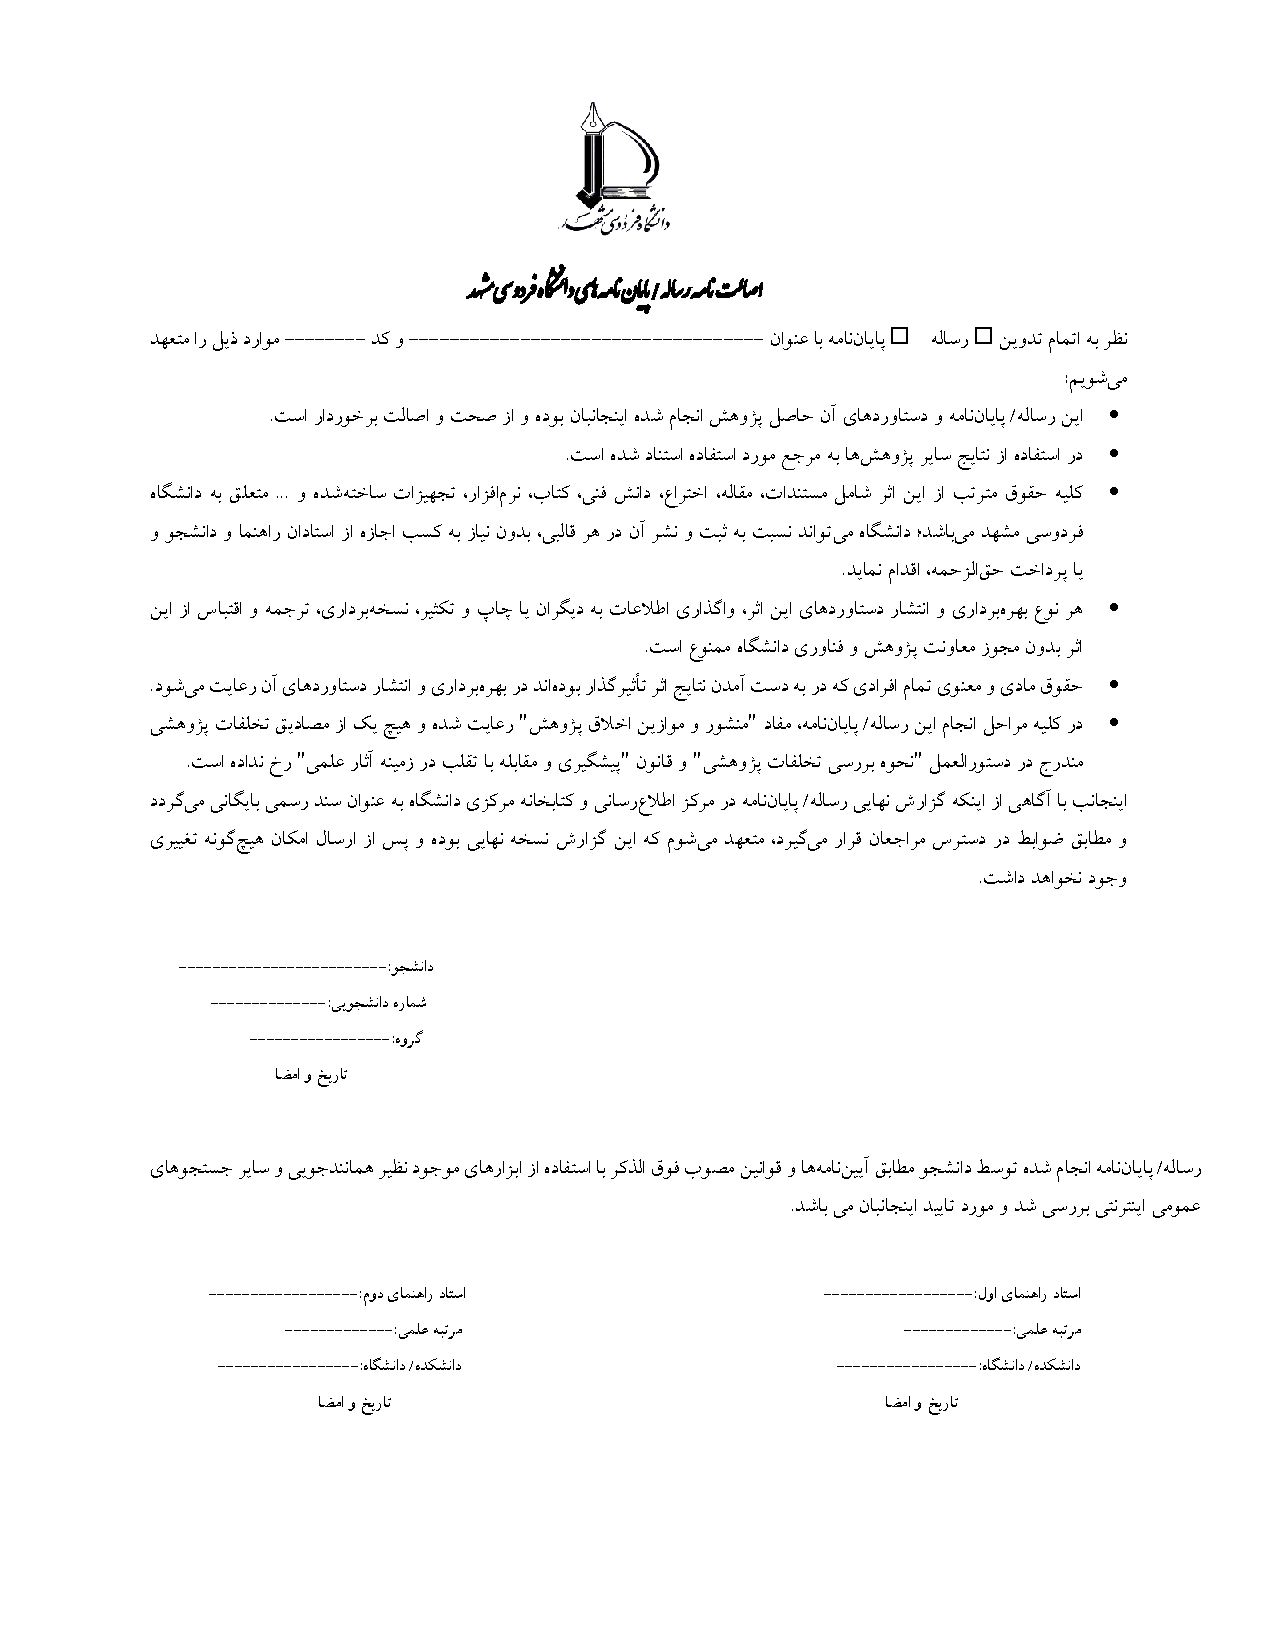
\includepdf{originality}
\presentation{1}{...}{...}{...}
\praise{1}{...}{...}{...}
\thanks{1}{...}{...}{...}
\end{verbatim}
\end{latin}

بخش دوم که مربوط به خودتان است را ما با راهنماهای متفاوت و مرتبط تکمیل کرده‌ایم. قبل از حذف آن‌ها سعی کنید پایان‌نامه خودتان را با همان فایل‌ها تکمیل کنید.

بخش سوم هم شامل فایل‌های \lr{appendix.tex}، \lr{refs.tex} و \lr{refs.bib} ست و بقیه اطلاعات مربوط به این بخش هم از همان فایل \lr{options.tex} خوانده می‌شود.

از اینجا به بعد کافی‌ست که تکه‌تکه قسمت‌های پایان‌نامه خودتان را جایگزین کنید.